\documentclass[UTF8]{ctexbeamer}
\usepackage{amsmath,amssymb,amsfonts}
\usepackage{graphicx}
\usepackage{pgfplots}
\pgfplotsset{compat=1.18}

\definecolor{themeBlue}{RGB}{27,89,149}
\definecolor{themeLight}{RGB}{234,244,255}
\setbeamercolor{structure}{fg=themeBlue}
\setbeamercolor{palette primary}{bg=themeBlue, fg=white}
\setbeamercolor{palette secondary}{bg=themeLight, fg=themeBlue}
\setbeamercolor{title}{fg=themeBlue}
\setbeamercolor{frametitle}{fg=themeBlue}
\setbeamercolor{block title}{bg=themeBlue, fg=white}
\setbeamercolor{block body}{bg=themeLight, fg=black}
\usetheme{Madrid}

\title{指数跟踪优化：Relax-L1稀疏模型与BIC筛选}
\author{杨昊霖、张宸铭}
\date{\today}

\begin{document}

\begin{frame}
  \titlepage
\end{frame}

\begin{frame}{研究路径}
  \begin{enumerate}
    \item 以Q6(b)基准模型为起点，建立经典跟踪有效前沿优化。
    \item 固定熵激励参数$\lambda_1$，引入Relax-L1稀疏惩罚。
    \item 遍历$\lambda_2$生成$(n,L)$序列。
    \item 使用BIC准则筛选最优$n$。
  \end{enumerate}
\end{frame}

\begin{frame}{基准模型（Q6(b)）}
  \[
  \min_{\boldsymbol{w}} \ \mathrm{Var}(\boldsymbol{w}^\top \boldsymbol{r} - r_M)
  \]
  \[
  \text{s.t. } \boldsymbol{w}^\top \boldsymbol{1} = 1,\quad \boldsymbol{w}^\top \boldsymbol{\mu} = \mu_0
  \]
  \vspace{0.3cm}
  \textbf{目标：} 最小化跟踪误差方差并满足全仓与均值约束。
\end{frame}

\begin{frame}{熵激励与Relax-L1稀疏}
  \[
  \min_{\boldsymbol{w}} \ \mathrm{Var}(\boldsymbol{w}^\top \boldsymbol{r} - r_M)
  - \lambda_1 \Big(-\sum_i w_i\ln w_i\Big) + \lambda_2 \|\boldsymbol{w}\|_1
  \]
  \begin{itemize}
    \item $\lambda_1$：权重分散激励（固定）。
    \item $\lambda_2$：稀疏惩罚（调节选股规模）。
  \end{itemize}
\end{frame}

\begin{frame}{两步法求解}
  \begin{block}{第一步：放松约束选股}
  移除全仓与均值约束，引入L1稀疏惩罚，得到候选成分股集合。
  \end{block}
  \begin{block}{第二步：全约束权重优化}
  在子集内恢复全仓、均值与非负约束，求解最终权重。
  \end{block}
\end{frame}

\begin{frame}{BIC准则}
  \[
  \mathrm{BIC}(n) = \ln(\mathrm{Var}(\boldsymbol{w}^\top \boldsymbol{r} - r_M)) + n\cdot \frac{\ln T}{T}
  \]
  \begin{itemize}
    \item $n$：选股数量。
    \item $T$：样本长度。
    \item 最小化BIC选取最优稀疏度。
  \end{itemize}
\end{frame}

\begin{frame}{BIC曲线示例}
  \begin{figure}
    \centering
    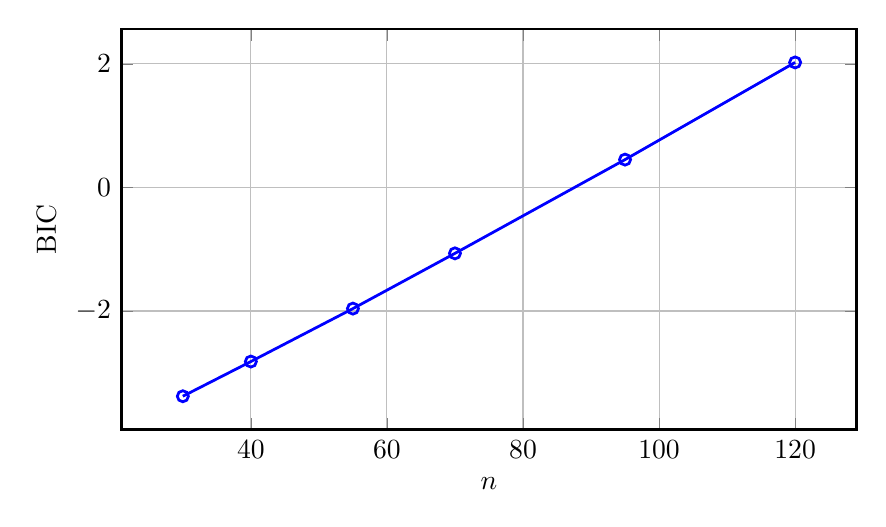
\begin{tikzpicture}
\begin{axis}[
width=0.9\linewidth,
height=0.55\linewidth,
grid=both,
xlabel={$n$},
ylabel={BIC},
line width=1pt,
]
\addplot+[mark=o, color=blue] coordinates {
(120, 2.022871)
(95, 0.450426)
(70, -1.066309)
(55, -1.960684)
(40, -2.817216)
(30, -3.378978)
};
\end{axis}
\end{tikzpicture}
  \end{figure}
\end{frame}

\begin{frame}{结论}
  \begin{itemize}
    \item Relax-L1两步法实现跟踪误差与组合稀疏度的平衡。
    \item 固定$\lambda_1$并调节$\lambda_2$生成$(n,L)$序列。
    \item BIC准则为成分股数量提供可解释选择。
  \end{itemize}
\end{frame}

\end{document}
